\documentclass[acmsmall,screen,review]{acmart}
\usepackage{booktabs}
\usepackage{siunitx}
\setcopyright{none}
\acmJournal{TOS}

\usepackage{array}
\begin{document}

\title{How KV Dies Decides How Flash Wears:\texorpdfstring{\\}{ }
Endurance and Provisioning of Hybrid CXL Memory for LLM KV Caches}

\author{Romyull Islam}
\email{mislam22@students.kennesaw.edu}
\affiliation{%
  \institution{Kennesaw State University}% department to be added
  \city{Kennesaw}
  \state{Georgia}
  \country{USA}}

\begin{abstract}
Flash is becoming a tier of the LLM key-value (KV) cache: NVIDIA's context-memory platform adds a
pod-level flash tier for KV, an SSD vendor has announced a platform for KV caching rated at 7 to more
than 10 drive writes per day, and hybrid CXL memory devices put a DRAM cache in front of a terabyte
or more of NAND. Whether that flash lasts depends on how much KV a serving node writes and how the
flash translation layer amplifies it, and we found no published study that gives these for a
hybrid CXL device.
We measure both with six production traces from two providers, a model of a hybrid device scaled
consistently to the prefill throughput of an 8-GPU node, and a flash translation layer validated
against closed forms and MQSim, and we check the key effects on a real NVMe drive. Three findings follow. First, how KV dies decides how flash wears: an
LRU prefix cache evicts in near write order and keeps write amplification at a median of 1.00, while
KV freed per request reaches 2.1 with TRIM and 5.2 without it at 7\% over-provisioning, the case on
CXL.mem, which has no TRIM; on a real 1\,TB drive the three cases slow sustained writes 0.98, 2.28 and
5.95 times. Second, the write rate itself is the wall: with second-hit admission TLC
lasts five years in only 10 of 108 cases, and 20 exceed even SLC. Third, admission control and lower KV
precision cut writes 2 to 20 and 2 to 4 times (BF16 at full prefill duty) without new hardware, and for request-scoped KV a discard command per finished request,
sent on the management path, lets the device drop dead KV from its DRAM and trim it, cutting flash
writes 3.4 to 9.1 times with commands as slow as 100\,ms; a real drive discards 1\,MiB to 4\,GiB in
0.5 to 81\,ms when idle. We turn the results into provisioning rules across flash type, KV precision, admission
and prefill duty.
\end{abstract}

\begin{CCSXML}
<ccs2012>
<concept><concept_id>10010583.10010600.10010607</concept_id>
<concept_desc>Hardware~Non-volatile memory</concept_desc><concept_significance>500</concept_significance></concept>
<concept><concept_id>10010520.10010521</concept_id>
<concept_desc>Computer systems organization~Architectures</concept_desc><concept_significance>300</concept_significance></concept>
</ccs2012>
\end{CCSXML}
\ccsdesc[500]{Hardware~Non-volatile memory}
\ccsdesc[300]{Computer systems organization~Architectures}
\keywords{CXL, hybrid memory, NAND flash, endurance, write amplification, KV cache, LLM serving}

\maketitle

\section{Introduction}
Long contexts, multi-turn chat and agents make LLM serving reuse prompt prefixes across requests, and serving systems
keep the KV cache of those prefixes beyond GPU memory to avoid recomputing
them~\cite{mooncake,lmcache,kvwild}. Two NVIDIA systems put flash below host memory. NVIDIA
Dynamo's KV block manager offloads KV from GPU memory to host memory and on to local
SSDs~\cite{dynamo_kvbm}, and NVIDIA's CMX context memory platform adds a pod-level,
Ethernet-attached flash tier built for KV~\cite{nvidia_cmx}. Hybrid CXL devices such as Samsung's
CMM-H attach flash as memory: a DRAM cache of 16 to 48\,GB sits in front of a terabyte or more of
NAND~\cite{cmmh,cmmh_hs}, and HyMCache~\cite{hymcache}, ITME~\cite{itme}, LM-CXD~\cite{lmcxd} and
TempoKV~\cite{tempokv} build KV caches on CXL-attached flash. These systems report time to first
token and throughput, and HyMCache and ITME also report hit rates. None measures wear: HyMCache and
TempoKV never discuss endurance, ITME discusses it only qualitatively, and LM-CXD aligns KV chunks
with erase blocks to avoid garbage collection without quantifying wear.

Wear limits such a device before capacity or bandwidth does. TLC flash endures about 1,000
program/erase cycles~\cite{cai_proc}, a KV cache writes every block it admits, and an eight-GPU node
that admits everything writes 3.3 to 15\,GB/s of new KV to flash (Section~\ref{sec:wear}). Vendors already see wear as the limit: ScaleFlux has
announced an SSD platform for KV caching rated at 7 to more than 10 effective drive writes per day
(DWPD), against 1 to 3 for mainstream TLC drives, and reports that KV blocks with different lifetimes
sharing flash blocks raise write amplification~\cite{scaleflux}. Work on on-package high-bandwidth
flash (HBF) answers parts of the question: on the Qwen-Bailian traces a flash KV tier writes 1.14 to
4.90 times more than it reads, 48 to 140\,TB per day per eight-GPU system, against a 21.7\,TB/day
TLC budget at write amplification 1~\cite{hbfsucks}; mixed KV lifetimes in one erase block drive
garbage-collection write amplification to about 30 on average for one model~\cite{hbflex}; and
placement, admission and endurance studies extend or assess HBF life (Section~\ref{sec:related}).
TRIM has been argued for CXL memory in general~\cite{trimcxl}. None of this models a DRAM-over-NAND CXL device,
contrasts the ways KV dies, sweeps flash type and KV precision, or divides the device among the
interleaved streams of a node.

We ask three questions. How much KV does a serving node write to flash per day? What decides write
amplification for KV? And which flash class, KV precision and admission policy let a device last
five years?

\begin{figure}[t]
\centering
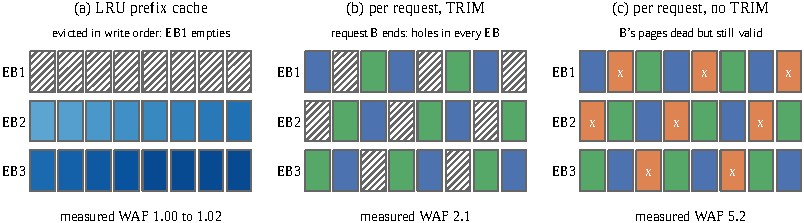
\includegraphics[width=\textwidth]{fig_concept.pdf}
\Description{Three panels of three erase blocks of eight pages each. In the LRU panel the first erase block is entirely invalid. In the TRIM panel, pages of one request are invalid in every erase block. In the no-TRIM panel, those pages are dead but still marked valid.}
\caption{How KV dies decides write amplification. Three erase blocks (EB) at garbage-collection
time; hatched pages are invalid. (a) An LRU prefix cache evicts nearly in write order (shades of
blue: write order), so whole erase blocks become invalid together and garbage collection copies
at most 2\% extra pages (write amplification 1.00 to 1.02). In (b) and (c), blue, orange and green pages belong to requests A, B and C.
(b) KV kept per request interleaves requests in every erase block; when request B ends and is
trimmed, every block has holes and its live pages must be copied. (c) CXL.mem has no TRIM, so B's
dead pages (x) stay valid and are copied too. Write amplification measured at 7\%
over-provisioning (Section~\ref{sec:waf}).}
\label{fig:concept}
\end{figure}

\textbf{Findings.}
\begin{enumerate}
\item \emph{How KV dies decides write amplification} (Fig.~\ref{fig:concept}). An LRU prefix cache
stays near 1 (median 1.00, at most 1.94 at 7\% over-provisioning); KV freed per request reaches 2.1
with TRIM and 5.2 without it, so CXL.mem's lack of TRIM costs 2.5 times. On a real NVMe drive the
three cases slow sustained writes 0.98, 2.28 and 5.95 times, and the missing TRIM costs 2.6 times
(Section~\ref{sec:waf}, Table~\ref{tab:ssd}).
\item \emph{The write rate itself is the wall.} Without admission control a node at full prefill
duty writes 280 to 1,290\,TB of BF16 KV to flash per day (Section~\ref{sec:wear}); with second-hit
admission TLC lasts five years in only 10 of 108 cases, a device rated 10 DWPD covers 40, and 20
exceed even SLC (Section~\ref{sec:prov}).
\item \emph{Admission control and KV precision cut writes without new hardware.} Second-hit and oracle admission
cut the writes 2 to 20 times with BF16 KV at full duty (up to 22 times over the sweep), and FP8 and
INT4 halve and quarter them; INT4 instead of BF16 moves 34
of 36 cases to a cheaper flash class. For a prefix cache, growing device DRAM from 16 to 256\,GB
changes per-node NAND writes by $-0.4$ to $+5.7\%$ with second-hit admission (Section~\ref{sec:prov}).
\item \emph{A discard per finished request repairs request-scoped KV.} Sent on the management path,
it lets the device drop dead KV from its DRAM and trim it, cutting flash writes 3.4 to 9.1 times
with commands as slow as 100\,ms; on a real drive a discard takes 0.5 to 81\,ms when the drive is
idle, but a 1\,MiB discard waits a median of 0.9\,s (up to 1.0\,s) behind queued writes
(Section~\ref{sec:discard}).
\item \emph{A shared pool gains 1 to 18\% in hits over cache-aware routing} that balances load (Section~\ref{sec:pool}).
\end{enumerate}

\textbf{Contributions.} (1) A trace-driven model of a hybrid device with consistent per-node scaling
(Section~\ref{sec:method}); (2) write amplification of KV measured with a flash translation layer
validated against Desnoyers' closed forms~\cite{desnoyers} and MQSim~\cite{mqsim}, and checked on a
real NVMe drive (Sections~\ref{sec:method} and~\ref{sec:waf}); (3) provisioning rules across flash
class, KV precision, admission and prefill duty for six traces and three models
(Section~\ref{sec:prov}); and (4) a per-request discard mechanism, the rate and address-space limits
it needs, and its latency on a real drive (Section~\ref{sec:discard}). Sections~\ref{sec:load} and~\ref{sec:pool} add when loading KV from the
device beats recomputing it and how much a shared pool gains; Section~\ref{sec:related} covers
related work and Section~\ref{sec:disc} the limitations.

\section{Background}
\label{sec:bg}
\textbf{Hybrid CXL memory.} A CXL Type-3 device exposes memory to the host over CXL.mem. A hybrid
device backs that memory with NAND and keeps a DRAM cache: the CMM-H prototype has a 16\,GB
8-way cache with 4\,KB blocks over a 1\,TB TLC SSD~\cite{cmmh}; a newer version has a 48\,GB cache
and reaches about 27\,GB/s when the working set fits in it and about 5\,GB/s when it does
not~\cite{cmmh_hs}. ITME's internal SSD-to-DRAM path measures 9 to 18\,GB/s, but its
FPGA prototype delivers under 1\,GB/s on cache misses~\cite{itme}. The host sees memory, not a block device:
CXL.mem has no TRIM, so the device learns that data is dead only when the host overwrites it.
Figure~\ref{fig:arch} shows the system we model.

\begin{figure}[t]
\centering
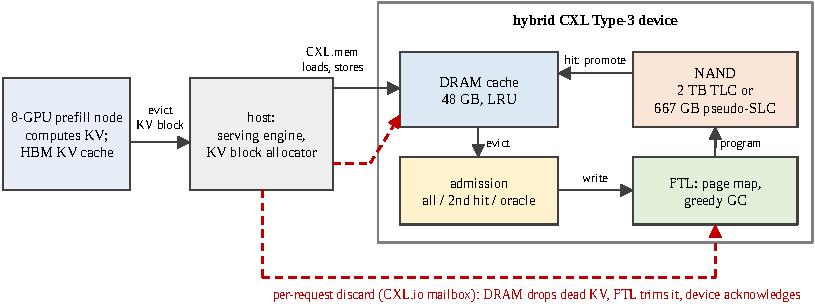
\includegraphics[width=\textwidth]{fig_arch.pdf}
\Description{A GPU node evicts KV blocks to the host, which writes them over CXL.mem into a hybrid device: a DRAM cache, an admission filter, a flash translation layer and NAND. A dashed path from the host carries a per-request discard over the CXL.io mailbox to the DRAM cache and the FTL.}
\caption{The modeled system. KV blocks evicted from GPU memory reach the device's DRAM cache over
CXL.mem; blocks evicted from DRAM that pass admission are written to NAND through the FTL, and NAND
hits are promoted to DRAM. The dashed path is the per-request discard of Section~\ref{sec:discard}.}
\label{fig:arch}
\end{figure}

\textbf{Flash endurance.} Enterprise drives are rated in drive writes per day (DWPD) over five
years. Read-intensive TLC drives are rated 1 DWPD and mixed-use TLC drives 3 DWPD (Samsung PM9A3,
Micron 7450 PRO and MAX, Kioxia CM7-R and CM7-V)~\cite{ds_samsung,ds_micron7450,ds_kioxia}. TLC run
as SLC, one bit per cell instead of three, is rated 35 random-write DWPD (Micron
XTR)~\cite{ds_micronxtr}, and a native SLC drive 50 DWPD (Solidigm D7-P5810)~\cite{ds_solidigm}.
Micron and Solidigm rate random 4\,KB writes; Micron rates 128\,KB sequential writes 1.7 to 4.4
times higher for the same 7450 drive~\cite{ds_micron7450}. Write amplification (WAF), the flash pages programmed per page written by the host,
multiplies the wear; with greedy garbage collection under uniform random writes it is 7.5 at
7\% over-provisioning and 2.4 at 28\%~\cite{desnoyers,vanhoudt}.

\textbf{KV caches.} Serving engines split a prompt into blocks of 16 to 512 tokens identified by a
hash of the prefix. A request reuses the longest cached prefix of its blocks and recomputes the
rest~\cite{vllm,mooncake}. A block is worth keeping only if a later request reuses it.

\section{Methodology}
\label{sec:method}

\begin{table}[t]
\caption{Configuration.}
\label{tab:config}
\small
\begin{tabular}{@{}>{\raggedright}p{3.3cm}>{\raggedright\arraybackslash}p{10.2cm}@{}}
\toprule
Node & 8 H100 GPUs at 989 dense BF16 TFLOP/s each and an assumed utilization of 0.5; prefill duty 100\%
(dedicated prefill node) or 30\% (node that also decodes) \\
Device & LRU DRAM cache of 48\,GB over LRU NAND: 2\,TB of TLC, or 667\,GB of the same NAND in
pseudo-SLC mode \\
Flash translation layer & page-mapped, greedy garbage collection into a separate block, 64\,MiB
erase blocks, 7\% or 28\% over-provisioning \\
Models & Llama-3.1-70B (GQA, 70.6B parameters, 320\,KiB of BF16 KV per token);
DeepSeek-V3~\cite{deepseekv3} (MLA,
37.6B active, 69\,KiB); Qwen2.5-7B (GQA, 7.6B, 56\,KiB) \\
KV precision & BF16; FP8 and INT4 halve and quarter the bytes per token \\
Admission to NAND & all; second hit; oracle \\
Five-year budgets & on a 2\,TB device: TLC at 1 DWPD (TLC-1), 2\,TB/day; TLC at 3 DWPD (TLC-3),
6\,TB/day; pseudo-SLC, 667\,GB at 35 DWPD, 23\,TB/day; SLC at 50 DWPD, 100\,TB/day \\
\bottomrule
\end{tabular}
\end{table}

\textbf{Traces.} Table~\ref{tab:traces} lists the six traces. Mooncake's conversation and
tool-agent traces cover one hour of Kimi traffic with 512-token blocks~\cite{mooncake}; the four
Qwen-Bailian traces cover two hours each of chat, API, coding and reasoning traffic with 16-token
blocks~\cite{bailian}. The share of blocks that are ever reused spans 6\% (API) to 47\% (chat).

\begin{table}[t]
\caption{Production traces. Blocks reused: share of unique blocks referenced again later.}
\label{tab:traces}
\resizebox{\textwidth}{!}{\begin{tabular}{lrrrrrrl}
\toprule
trace & requests & hours & block tokens & mean input & mean output & unique blocks & blocks reused \\
\midrule
Bailian API & 172800 & 2.00 & 16 & 915 & 92 & 3830390 & 6\% \\
Bailian thinking & 10812 & 2.00 & 16 & 4763 & 3651 & 1735015 & 14\% \\
Mooncake tool-agent & 23608 & 0.98 & 512 & 8596 & 182 & 183300 & 22\% \\
Mooncake conversation & 12031 & 0.98 & 512 & 12035 & 343 & 182790 & 24\% \\
Bailian coder & 43011 & 2.00 & 16 & 5748 & 808 & 5202517 & 39\% \\
Bailian chat & 43058 & 2.00 & 16 & 2331 & 430 & 2530337 & 47\% \\
\bottomrule
\end{tabular}
}
\end{table}

\textbf{Device model.} The device has an LRU DRAM cache (48\,GB) over an LRU NAND tier (2\,TB,
or 667\,GB for the same NAND in pseudo-SLC mode). Requests read their blocks as a prefix: blocks
found in DRAM or NAND are hits until the first miss, after which blocks are recomputed and written
to DRAM. A block read from NAND is promoted to DRAM and stays in NAND. A block evicted from DRAM
is written to NAND if the admission policy accepts it and NAND does not hold it. We compare three
policies: \emph{all}; \emph{second hit}, which admits blocks referenced at least twice so far,
the cache-on-second-hit rule of content delivery networks~\cite{secondhit} (Flashield likewise
filters flash admission in DRAM, with a learned predictor~\cite{flashield}); and \emph{oracle},
which admits a block only if it will be referenced again, a bound on what a reuse predictor can
know. With BF16 KV at full prefill duty, second hit writes 0.73 to 1.13 times as much as the oracle
(0.71 to 2.0 over the whole sweep) and loses 2 to 41\% of its hits (median 15\%), because the
second reference arrives after the block has left the DRAM cache. FP8 and INT4 KV also
fit 2 and 4 times as many blocks in the device.

\textbf{Per-node scaling.} A trace is one stream of users; a node serving $S$ times its traffic
interleaves $S$ independent streams, which stretches reuse distances $S$-fold on average. We model the
node by dividing the device's DRAM and NAND by $S$ and find $S$ as a fixed point:
\begin{equation}
G \cdot F \cdot u \cdot d \,/\, (2P) = S \cdot m(C/S),
\end{equation}
where the left side is the node's prefill throughput in tokens per second ($G=8$ H100 GPUs of
$F=989$ dense TFLOP/s at an assumed utilization $u=0.5$, prefill duty $d$, $P$ active parameters;
the linear term only, which overstates the rate by ignoring attention) and $m(C/S)$
is the trace's miss rate in tokens per second on a device of capacity $C/S$. The NAND write rate
is $S$ times the trace's. $S$ is 0.3 to 7 for Llama-3.1-70B, 0.5 to 14 for DeepSeek-V3 and 2.4
to 67 for Qwen2.5-7B. We assume a prefill duty of 100\% for a dedicated prefill node and 30\% for a
node that also decodes.

\textbf{Flash translation layer.} The NAND write stream (one entry per block written, naming the
slot it overwrites) drives a page-mapped FTL with greedy garbage collection that, like MQSim,
writes relocated data to its own block, with 64\,MiB erase blocks (as many whole KV blocks as fit)
and 7\% or 28\% over-provisioning. Table~\ref{tab:ftl} validates the FTL against the closed forms
for uniform random writes~\cite{desnoyers}, and Table~\ref{tab:mqsim} against MQSim~\cite{mqsim},
a validated SSD simulator (patched to fix a crash; runs that complete unpatched give identical
results), on three KV write streams: two LRU streams from a reduced device on the Bailian chat
trace and the request-scoped stream. With MQSim's reserve of 10 free blocks the two agree within
4.5\% on the KV streams and within 11.3\% on uniform random writes. When a trace writes less than four
times the NAND capacity, we append copies of it with new block identifiers (new users), at most 12
copies in all, for the write-amplification measurement only; for 25\% of the 2\,TB cases and 10\% of
the 667\,GB cases the stream still writes less than three times the capacity and we take write
amplification as 1. With 512-token
Mooncake blocks, at most one KV block of Llama-3.1-70B, or of DeepSeek-V3 with BF16 KV, fits in an
erase block; these cases (15\% of the sweep) have write amplification 1 by construction.

\begin{table}[t]
\caption{FTL validation: uniform random overwrites, 40{,}000 units, 64 units per erase block.
Effective over-provisioning excludes the reserved free blocks.}
\label{tab:ftl}
\small
\begin{tabular}{llrrr}
\toprule
over-provisioning & victim & effective OP & simulated WAF & closed form \\
\midrule
7\% & fifo & 0.064 & 8.289 & 8.486 \\
7\% & greedy & 0.064 & 7.424 & 7.530 \\
28\% & fifo & 0.274 & 2.515 & 2.523 \\
28\% & greedy & 0.274 & 2.435 & 2.440 \\
\bottomrule
\end{tabular}

\end{table}

\begin{table}[t]
\caption{Write amplification on exported KV write streams and on uniform random writes (64 units
per erase block): MQSim and our FTL with MQSim's 10 reserved free blocks. MQSim collects up to 10
victims concurrently; given 9 more physical blocks to offset them, MQSim gives 7.52 on uniform
writes at 7\% (our FTL: 7.91 with its 10 reserved blocks) and 5.36 on the request-scoped stream.}
\label{tab:mqsim}
\small
\begin{tabular}{llrrl}
\toprule
KV write stream & OP & MQSim & this FTL & difference \\
\midrule
LRU cache, oracle admission & 7\% & 1.043 & 1.065 & +2.1\% \\
LRU cache, oracle admission & 28\% & 1.000 & 1.000 & +0.0\% \\
LRU cache, admit all & 7\% & 1.004 & 1.005 & +0.1\% \\
LRU cache, admit all & 28\% & 1.000 & 1.000 & +0.0\% \\
request-scoped, no TRIM & 7\% & 5.649 & 5.397 & -4.5\% \\
request-scoped, no TRIM & 28\% & 1.968 & 1.975 & +0.3\% \\
uniform random (reference) & 7\% & 8.917 & 7.907 & -11.3\% \\
uniform random (reference) & 28\% & 2.500 & 2.461 & -1.6\% \\
\bottomrule
\end{tabular}

\end{table}

\textbf{Request-scoped KV.} To contrast how KV dies, we also drive the FTL with KV that lives as long
as its request. Each request of the Bailian thinking trace, at its real arrival time and output
length, writes its decode KV one 16-token block at a time at 30 tokens/s and frees all of it when it
ends. The device's logical space equals the peak live KV, and freed slots are reused in FIFO order.
With TRIM, freed blocks are invalidated at once; without it, as on CXL.mem, they stay valid in the
FTL until the host overwrites their slot. Erase blocks hold 64 KV blocks, as in the prefix-cache
comparison on the same trace; this measures write amplification and does not depend on the model's
KV size.

\textbf{Budgets.} A case fits a flash class if its NAND writes, including write amplification at
7\% over-provisioning for TLC-1 and 28\% otherwise, stay within the budget of
Table~\ref{tab:config}.

\section{Per-node NAND writes exceed TLC budgets}
\label{sec:wear}
Figure~\ref{fig:wear} shows the NAND writes per node at full prefill duty with BF16 KV. Admitting
everything writes 281 to 319\,TB/day for DeepSeek-V3, 714 to 793 for Llama-3.1-70B and 1,174 to
1,291 for Qwen2.5-7B, 47 to 646 times the TLC budgets and above any SLC budget, and 1.3 to 5.3
times more than the device ever reads back. Second-hit and oracle admission cut this by 2 to 20
times, most for the API trace, where only 6\% of blocks are reused. Per node, small models write
the most (1.6 to 2.3 times Llama-3.1-70B): their nodes prefill 9.3 times as many tokens, which
outweighs their 5.7 times smaller KV. MLA writes 2.5 to 2.9 times less than Llama-3.1-70B: its KV is
4.7 times smaller, but its node prefills 1.9 times as many tokens.

\begin{figure}[t]
\centering
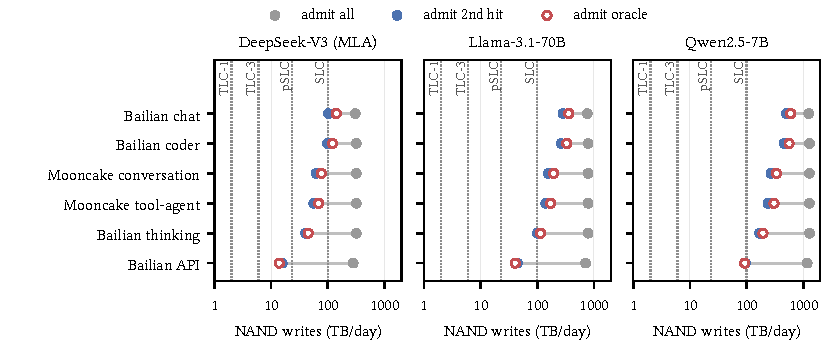
\includegraphics[width=\textwidth]{fig_wear.pdf}
\Description{Dot plot of NAND terabytes written per day per node for each trace, model and admission policy, with vertical dotted lines for the five-year budgets of TLC, pseudo-SLC and SLC devices.}
\caption{NAND writes per node at full prefill duty with BF16 KV and 28\% over-provisioning, by trace
and admission policy. Dotted lines are the five-year budgets of a 2\,TB device (pSLC:
pseudo-SLC).}
\label{fig:wear}
\end{figure}

Two common shortcuts understate wear. Computing hit rates on a full device and multiplying the
write rate by the node's throughput, without dividing the device by $S$, understates the writes of
small models by up to 1.8 times (Qwen2.5-7B, API trace, oracle admission). Taking write
amplification as 1, as HBF Sucks? does~\cite{hbfsucks}, misses a factor of up to 1.55 on the 2\,TB
device and 1.94 on the pseudo-SLC device at 7\% over-provisioning even for an LRU cache, and of 5.2
for request-scoped KV without TRIM (Section~\ref{sec:waf}).

\textbf{Takeaway.} Admitting every block, a node writes 280 to 1,290\,TB of KV per day, 47 to 646
times the five-year budget of a 2\,TB TLC device rated 1 or 3 DWPD.

\section{Write amplification depends on how KV dies}
\label{sec:waf}
Figure~\ref{fig:waf} (left) shows the measured write amplification over all prefix-cache
configurations. The median is 1.00. At 28\% over-provisioning it never exceeds 1.07 on the
2\,TB device and 1.18 on the smaller pseudo-SLC device; at 7\% oracle admission reaches 1.55 on the
2\,TB device and 1.94 on the pseudo-SLC device (second hit: 1.34 and 1.66): the hits it keeps refresh
blocks in the NAND tier's
LRU order, so blocks no longer die in the order they were written.

\begin{figure}[t]
\centering
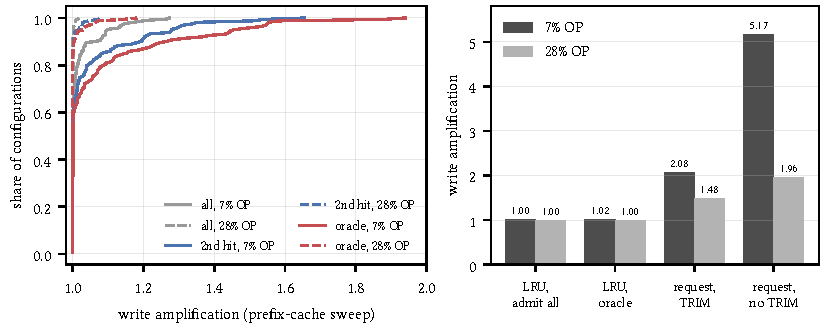
\includegraphics[width=\textwidth]{fig_waf.pdf}
\Description{Left, distribution of measured write amplification over the sweep; right, write amplification for an LRU prefix cache and for request-scoped KV with and without TRIM.}
\caption{Left: distribution of write amplification over the sweep. Right: write amplification by
how KV dies, on the Bailian thinking trace with 64 KV blocks per erase block.}
\label{fig:waf}
\end{figure}

The right panel isolates the cause. An LRU cache evicts blocks nearly in write order, so whole
erase blocks die together and garbage collection copies at most 2\% extra pages: write
amplification 1.00 to 1.02. HiFC reports 1.02 from host-side SMART counters for append-only writes on a consumer
drive~\cite{hifc}. If instead KV is kept per request and freed when the request ends, concurrent requests interleave
their blocks in every erase block and end at different times. This is how a tier behaves when it
holds the KV of live requests rather than a prefix cache: preempted or swapped requests~\cite{vllm},
agent sessions paused on tools, and decode KV of long reasoning requests offloaded while they run;
ScaleFlux names the same pattern, KV invalidated asynchronously across sessions~\cite{scaleflux}.
We model the last case on the Bailian thinking trace (Section~\ref{sec:method}): write amplification is 2.1 at 7\% over-provisioning
with TRIM. CXL.mem has no TRIM, so freed blocks stay valid in the FTL until the host reuses their
addresses, and write amplification rises to 5.2, 2.5 times the TRIM case. HBFlex reports an
average of about 30 for DeepSeek-V4-Pro KV pages of mixed lifetimes sharing HBF erase
blocks~\cite{hbflex}; the mechanism is the same, on a different device, model and mapping
granularity. Lee et al.\ argue for TRIM in CXL memory in general and, with an analytical model
validated in an FTL simulator, estimate a write-amplification cut of up to 19.7\% for Azure VM
traces at 10\% spare space~\cite{trimcxl}; for request-scoped KV the cut is 60\%, because whole
requests die at once. NVMe SSDs can also separate lifetimes with lifecycle-aware placement, which
ScaleFlux reports more than halved write amplification for KV in preliminary
tests~\cite{scaleflux}; SPLASH gives each request its own HBF region and erases it as a
unit~\cite{splash}, and NVMe Flexible Data Placement lets a host group data by lifetime, which cuts
device write amplification for flash caches and databases~\cite{fdp_cachelib,fdp_promise}. All three need control of flash placement that CXL.mem does not give the host. A hybrid CXL
device that stores request-scoped KV therefore needs either 28\%
over-provisioning, which still leaves write amplification at 2.0, or a way for the host to declare data dead, and a serving engine that frees KV
in LRU order keeps write amplification at 1.00 to 1.02.

\textbf{On a real drive.} We replay the LRU stream of Table~\ref{tab:mqsim} (Bailian chat, admit
all) and the two request-scoped streams on a 1\,TB NVMe drive (WD SN580E in a SanDisk
Extreme enclosure, attached over USB, TRIM passed through as UNMAP), with each logical unit
mapped to an equal share of the whole drive (7.1\,MB per unit for the request-scoped streams, 19.7\,MB
for the LRU stream), so the drive's own spare area is the only over-provisioning. Before each stream the
drive is trimmed and written once sequentially; each KV stream then writes 1.5 times the drive's
capacity with direct I/O. The drive does not report NAND writes, so we use the standard proxy: once the drive
is full, garbage collection bounds sustained write bandwidth, and the slowdown against sequential
overwrites tracks write amplification. Table~\ref{tab:ssd} gives the median bandwidth over the last
third of each run. The drive orders the streams as the FTL does: the LRU stream writes as fast as
sequential overwrites (slowdown 0.98), request-scoped KV slows writes 2.28 times with TRIM and 5.95
times without, against 2.08 and 5.17 simulated, and the missing TRIM costs 2.6 times (2.5 simulated).
Uniform random overwrites, for reference, slow writes 8.93 times against a greedy closed form of 7.53;
the real drive runs 10 to 19\% above the simulated values for every stream that needs garbage
collection.

\begin{table}[t]
\caption{Real drive (1\,TB WD SN580E over USB): steady host write bandwidth with the drive full,
slowdown against sequential overwrites, and the write amplification of our FTL for the same stream
at 7\% over-provisioning (uniform random: greedy closed form). One run per stream; median and
interquartile range of 10-second samples over the last third of the run.}
\label{tab:ssd}
\small
\begin{tabular}{lrrrr}
\toprule
write stream & written (TB) & steady MB/s & slowdown & simulated WAF \\
\midrule
sequential overwrite & 1.00 & 393 & 1.00 & 1.00 \\
LRU prefix cache, admit all & 1.50 & 400 & 0.98 & 1.00 \\
request-scoped, TRIM & 1.50 & 172 & 2.28 & 2.08 \\
request-scoped, no TRIM & 1.50 & 66 & 5.95 & 5.17 \\
uniform random & 1.03 & 44 & 8.93 & 7.53 \\
\bottomrule
\end{tabular}

\end{table}

\textbf{Takeaway.} An LRU prefix cache keeps write amplification at 1.00 to 1.02; request-scoped KV
reaches 2.1 with TRIM and 5.2 without it, and a real drive slows sustained writes 2.28 and 5.95 times
for those two cases.

\section{Traffic, precision and admission decide the flash class}
\label{sec:prov}
Figure~\ref{fig:prov} gives the cheapest flash class that lasts five years with second-hit
admission. Four rules follow.
\begin{enumerate}
\item \emph{Admission control is mandatory.} Admitting everything never fits TLC, fits pseudo-SLC in
only 4 of 54 cases, all DeepSeek-V3 with INT4 KV at partial prefill duty, and at full prefill duty fits
nothing in 48 of 54 cases.
\item \emph{Workload decides the flash class.} TLC fits API-like traffic at partial prefill duty
(6 of 9 cases), but reasoning traffic only in 1 of 9 and interactive traffic (chat, coding,
conversation and agent) only in 2 of 36, all DeepSeek-V3 with INT4 KV. Interactive
traffic needs pseudo-SLC or SLC, and 16 of its 36 cases at full prefill duty (and 2 of 36 at partial
duty) exceed even 100\,TB/day.
\item \emph{KV precision is worth one flash class.} FP8 halves and INT4 quarters the NAND
writes (0.49 and 0.24 times BF16 on average); INT4 instead of BF16 moves 33 of 36 trace, model and
duty cases down exactly one class, one case two classes and two cases none.
\item \emph{Attention architecture changes the write rate.} With second-hit admission, MLA
(DeepSeek-V3) sends 2.3 to 2.9 times less KV to NAND than GQA Llama-3.1-70B per node, and the 7B GQA
model sends the most in all 36 cases.
\end{enumerate}
Drives announced for KV caching at 7 to more than 10 DWPD~\cite{scaleflux} would cover, at 10 DWPD
(20\,TB/day on a 2\,TB device), 31 of the 54 cases at partial prefill duty and 9 of 54 at full duty with
second-hit admission; at 7 DWPD, 21 and 4. Using the 1.7 times higher sequential rating for TLC moves 9 of the 108 cases from pseudo-SLC to
TLC; interactive traffic then fits TLC in 6 of 36 cases at partial duty, still all DeepSeek-V3, now
with FP8 or INT4 KV. Pseudo-SLC's smaller capacity (667\,GB) lowers the hit share by a median of 1.4 points
and leaves the median write rate unchanged. A second wall is bandwidth: 7\% of the
cases (22 of 324) need more than the about 5\,GB/s that the 48\,GB CMM-H sustains when its working
set does not fit in its DRAM cache~\cite{cmmh_hs}, all of them with admit-all or Qwen2.5-7B.

\textbf{Device DRAM size.} Growing the device's DRAM cache from 16 to 256\,GB (Bailian API, chat
and thinking traces, Llama-3.1-70B and DeepSeek-V3, BF16, full duty, second-hit and oracle
admission) changes the per-node NAND writes by $-0.4$ to $+5.7\%$ with second-hit admission and by
$-32$ to $0\%$ with oracle admission, while the share of hits served from DRAM rises from 0.24--0.49 to
0.35--0.90. A larger DRAM cache serves more hits from DRAM but does not extend lifetime: with $S$ interleaved streams, even 256\,GB
of DRAM evicts a block before its next reference, so second-hit admission writes it to NAND anyway.

\begin{figure}[t]
\centering
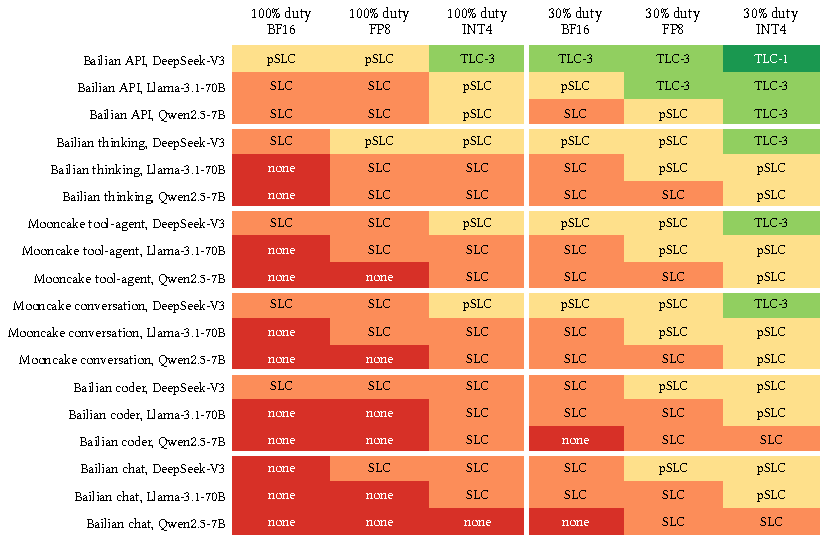
\includegraphics[width=\textwidth]{fig_prov.pdf}
\Description{A colored grid with eighteen rows, one per trace and model, and six columns, one per prefill duty and KV precision; each cell names the cheapest flash class that lasts five years.}
\caption{Cheapest flash class that lasts five years with second-hit admission, by trace, model,
prefill duty and KV precision. TLC-1 and TLC-3: TLC at 1 and 3 DWPD; pSLC: pseudo-SLC; none: above
100\,TB/day.}
\label{fig:prov}
\end{figure}

\textbf{Takeaway.} With second-hit admission, TLC lasts five years in 10 of 108 cases; INT4 KV moves 34
of 36 trace, model and duty cases to a cheaper flash class.

\section{Telling the device that KV is dead}
\label{sec:discard}
Request-scoped KV wastes flash twice on CXL.mem: dead blocks that device DRAM evicts are written to
NAND, and once there they stay valid until the host reuses their address. The serving engine knows
when a request ends. We evaluate a per-request discard. When a request ends, the
engine sends one command that names the request's blocks; the device drops their copies from its
DRAM without writing them back, trims them in the FTL and acknowledges. The host reuses a block's
address only after the acknowledgment, so a late discard never hits new data, the hazard Lee et al.\
point out for TRIM over CXL.io~\cite{trimcxl}. One command per finished request is 1.5
per second on the Bailian thinking trace, and at most 101 per second when the trace is scaled
to a node ($S \le 67$ in our sweep). The management path (a CXL.io mailbox command) is fast enough
if a command completes in under 10\,ms or names every request that ended while the previous command
ran, and CXL.mem needs no change. CXL already
defines a Media Operations mailbox command (opcode 4402h) whose Zero and Sanitize classes act on a
device address range~\cite{cxl40}, but Linux permits it only on ranges outside committed decoders, to
avoid corrupting active mappings~\cite{linux_mediaop}: it clears memory taken out of use, not KV that
dies while the memory stays mapped. The discard evaluated here could be added as another class of
that command. Lee
et al.\ propose TRIM as a privileged, asynchronous CXL.io command issued by the operating system or
by applications through a system call, and leave the initiator layer, granularity and frequency
open~\cite{trimcxl}; here the initiator is the serving
engine, and the DRAM drop adds to the trim.

\textbf{Method.} We use the request-scoped stream of Section~\ref{sec:method} with a write-back LRU
DRAM cache of 10\% or 25\% of the peak live KV in front of the FTL (7\% over-provisioning).
Discards queue on one serial channel and take 1\,ms to 10\,s each. After each block it writes, a
request reads 0, 1 or 4 of its earlier blocks at random, as sparse attention over offloaded KV would;
a read that misses DRAM fetches the block from NAND as a clean copy.

\begin{table}[t]
\caption{Flash page programs per KV block written by the host (NAND writes times write
amplification), request-scoped KV on the Bailian thinking trace, 7\% over-provisioning.}
\label{tab:discard}
\small
\begin{tabular}{rrrrrr}
\toprule
DRAM / live KV & reads per write & no discard & 1\,ms & 100\,ms & 1\,s (overloaded) \\
\midrule
10\% & 0 & 5.12 & 1.05 & 1.05 & 2.60 \\
10\% & 1 & 5.20 & 1.28 & 1.28 & 3.01 \\
10\% & 4 & 5.22 & 1.55 & 1.55 & 3.55 \\
25\% & 0 & 4.40 & 0.48 & 0.48 & 1.53 \\
25\% & 1 & 4.84 & 0.63 & 0.63 & 1.83 \\
25\% & 4 & 5.24 & 0.86 & 0.86 & 2.31 \\
\bottomrule
\end{tabular}
\end{table}

\textbf{Results.} With 1 to 100\,ms per command, discards cut flash programs by 3.4 to 9.1 times
(Table~\ref{tab:discard}); the result is the same at 1\,ms and at 100\,ms. Two effects add up.
Dropping dead copies from DRAM cuts NAND writes by 17 to 57\%, more with more DRAM and fewer reads,
and trimming cuts write amplification from 4.9--5.3 to 1.26--1.87. Addresses waiting for an
acknowledgment peak at 3.5\% of the peak live KV, but they peak when live KV is low: with 1\% extra
address space no allocation stalls at 1 to 100\,ms per command. The command channel fails only when completions per second times the command latency
exceed 1: at 1\,s per command and 1.5 completions per second the queue grows without bound, the
host stalls on 9,965 allocations and the gain falls to 1.5 to 2.9 times. At node scale (101 completions per second) a
command must therefore take under 10\,ms or cover the requests that ended while the previous one ran. On this trace the peak live KV
is 731\,GB for Llama-3.1-70B and 157\,GB for DeepSeek-V3, so 10 to 25\% of it is 16 to 39\,GB of
device DRAM for DeepSeek-V3, within CMM-H's 48\,GB, but 73 to 183\,GB for Llama-3.1-70B. For a
prefix cache with second-hit admission, 16 to 256\,GB of device DRAM changes per-node NAND writes by
$-0.4$ to $+5.7\%$ (Section~\ref{sec:prov}); DRAM saves flash only when the device learns what is
dead. This study uses a shorter request-scoped stream (2.18M block writes against 2.46M), so its
write amplification without discards is 5.1 to 5.3 rather than 5.17.

\textbf{Discard latency on a real drive.} On the drive of Table~\ref{tab:ssd}, a discard of a freshly
written range takes a median of 0.5\,ms for 1\,MiB, 3.0\,ms for 64\,MiB, 35\,ms for 1\,GiB and
81\,ms for 4\,GiB with the drive otherwise idle, within the 1 to 100\,ms we assume. Behind a
stream of 24\,MiB writes, ranges of 16\,MiB to 4\,GiB take 22 to 77\,ms, but a 1\,MiB discard waits
0.9\,s for the writes queued ahead of it. A device that implements the discard should therefore batch
the blocks of finished requests into large ranges, or give the command priority over queued writes.

\textbf{Takeaway.} A discard per finished request cuts flash programs of request-scoped KV 3.4 to 9.1
times at up to 100\,ms per command, and a real drive completes one in 0.5 to 81\,ms when idle.

\section{Loading beats recomputing above a bandwidth threshold}
\label{sec:load}
A hit served from the device pays only if loading the KV is faster than recomputing it. Recomputing
$n$ tokens on the node takes $t(n) = (2Pn + Lwn^2)/(G F u)$, with $w$ the attention width; loading
takes $n b / B$ for $b$ bytes of KV per token over a path of $B$ bytes per second. The break-even
bandwidth $B^* = nb/t(n)$ (Figure~\ref{fig:load}) falls with context length because attention makes
recompute superlinear; the trade-off itself is formalized in~\cite{restore_recompute,pykvcache}.
On 8 H100 GPUs, hits served from the device's DRAM cache (about 27\,GB/s~\cite{cmmh_hs}) always
pay. Hits from NAND (about 5\,GB/s) pay for DeepSeek-V3 at every precision, for Llama-3.1-70B only
with FP8 or INT4 KV, and for Qwen2.5-7B only with INT4. On B200 GPUs the break-even rises 2.3 times;
NAND hits then pay only for DeepSeek-V3 with FP8 or INT4 KV (BF16 only at 32K tokens) and for
Llama-3.1-70B with INT4 KV at 8K and 32K tokens. Lower KV precision thus helps twice: it cuts writes and
makes NAND hits worth serving.

\begin{figure}[t]
\centering
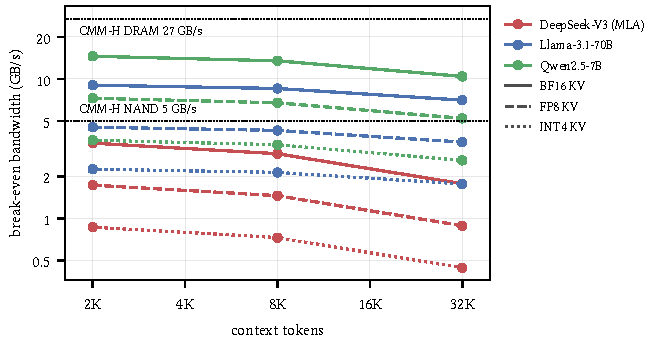
\includegraphics[width=0.8\textwidth]{fig_load.pdf}
\Description{Break-even load bandwidth versus context length for each model and KV precision on H100 nodes, with horizontal lines for the device's DRAM and NAND bandwidth.}
\caption{Bandwidth above which loading KV beats recomputing it on 8 H100 GPUs, with measured
device bandwidths.}
\label{fig:load}
\end{figure}

\textbf{Takeaway.} On 8 H100 GPUs, hits from the device's DRAM always pay; hits from NAND pay for
DeepSeek-V3 at every precision, for Llama-3.1-70B only with FP8 or INT4 KV, and for Qwen2.5-7B only
with INT4.

\section{A shared pool adds little over load-balanced routing}
\label{sec:pool}
A CXL pool shared by prefill hosts (4 to 16 in our runs) holds each block once and serves every host; per-host
caches duplicate popular blocks. Figure~\ref{fig:pool} compares a pool with per-host caches under
random and cache-aware routing; cache-aware routing sends a request to the host with the longest
cached prefix unless that host's load exceeds the mean by more than 25\%. Over 4 to 16 hosts and
total capacities of 2 to 50\% of the unique blocks, the pool hits 1.05 to 4.5 times as often as
random routing and writes 1.03 to 1.9 times fewer blocks, but beats cache-aware routing by only
1 to 18\% in hits and 1 to 9\% in writes. Mooncake reports up to 136\% more hits for its global
pool than for per-node local caches with prefix-aware routing, on 10 prefill nodes of 3M tokens
each~\cite{mooncake}. Reproducing that
setup, the pool gains 3 to 10\% when the scheduler allows 5 to 100\% imbalance, 15 to 43\% when it
balances exactly (Figure~\ref{fig:pool}, right), and 165\% when it ignores load (off the plot). The
scheduler's balance limit alone moves the pool's gain from 3 to 165\%. In NAND writes, the pool saves
1 to 9\% over cache-aware routing.

\textbf{Takeaway.} Against load-balanced, cache-aware routing, a shared CXL pool gains 1 to 18\% in
hits and 1 to 9\% in writes.

\begin{figure}[t]
\centering
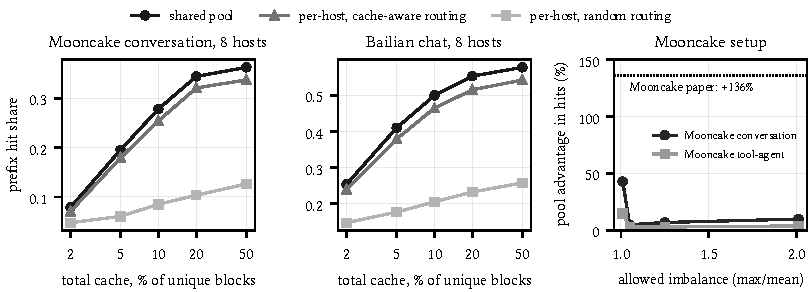
\includegraphics[width=\textwidth]{fig_pool.pdf}
\Description{Prefix hit share of a shared pool versus per-host caches under random and cache-aware routing, and the pool's advantage as the allowed load imbalance varies.}
\caption{Prefix hit share of a shared pool and of per-host caches (8 hosts), and the pool's
advantage at Mooncake's scale as the scheduler's allowed imbalance varies.}
\label{fig:pool}
\end{figure}

\section{Related work}
\label{sec:related}
\textbf{Flash as a KV tier.} HBF Sucks? characterizes a flash KV tier on the Qwen-Bailian traces,
writing 1.14 to 4.90 times more than it reads at an assumed write amplification of
1~\cite{hbfsucks}. Son et al.\ find endurance a critical challenge when all KV is written to
HBF~\cite{son_hbf}, while Kyung et al.\ find the lifetime acceptable for KV with high read-to-write
ratios~\cite{kyung_hbf}. HBFlex packs KV pages by lifetime to cut garbage-collection write
amplification~\cite{hbflex}, Lachesis places KV across HBM and HBF by lifetime~\cite{lachesis}, an
LRU-K admission policy extends HBF life for generative recommendation~\cite{huawei_hbf}, and request
admission does so for LLM serving~\cite{berkeley_hbf}. SPLASH gives each request its own HBF region,
erased as a unit~\cite{splash}, and HiFC runs a KV cache in pseudo-SLC on a consumer
SSD~\cite{hifc}. Industry platforms add flash tiers for KV~\cite{nvidia_cmx,dynamo_kvbm} and drives
rated for it~\cite{scaleflux}. These target on-package HBF or block SSDs; we model a hybrid CXL
device, whose DRAM cache and missing TRIM change both the write stream and its amplification.

\textbf{KV caches on hybrid CXL memory.} HyMCache~\cite{hymcache}, ITME~\cite{itme},
TempoKV~\cite{tempokv} and LM-CXD~\cite{lmcxd} build KV caches on CXL-attached flash and evaluate
latency and throughput. Two studies measure CMM-H~\cite{cmmh,cmmh_hs}, and Cylon emulates CXL-attached
SSDs~\cite{cylon}.

\textbf{Flash management.} Greedy garbage collection under uniform writes has closed
forms~\cite{desnoyers,vanhoudt}, and MQSim simulates multi-queue SSDs~\cite{mqsim}. Lee et al.\
argue for TRIM in CXL memory and model its effect on VM workloads~\cite{trimcxl}. Relaxed retention
trades data lifetime for endurance~\cite{warm}. Caching objects only on their second
access~\cite{secondhit}, or admitting them to flash by a learned
predictor~\cite{flashield,baleen}, reduces writes in other caches. NVMe Flexible Data Placement
separates data by lifetime on block SSDs~\cite{fdp_cachelib,fdp_promise}; CXL.mem has no
equivalent. For LLM prefix caches, recency dominates reuse, so LRU is hard to beat and one-hit
prefixes are best demoted early~\cite{fancy_eviction}, which matches the near-write-order eviction
and second-hit admission we study; compressing KV reduces the bytes a flash device must
endure~\cite{flash_inference}.

\textbf{KV reuse, pooling and recomputation.} KVCache-in-the-Wild characterizes KV reuse in
production~\cite{kvwild}; Mooncake and TokenLake pool KV across nodes~\cite{mooncake,tokenlake};
LMCache keeps KV beyond GPU memory~\cite{lmcache}; and the choice between loading and recomputing KV
is modeled and measured in~\cite{restore_recompute,pykvcache}.

\section{Discussion and limitations}
\label{sec:disc}
\textbf{Scaling.} Modeling a node as $S$ interleaved copies of a trace assumes independent users;
real routing can concentrate a conversation on one node, which shortens reuse distances and favors
the cache. The traces cover one to two hours, so daily load cycles enter only through the two prefill
duties (30\% and 100\%). $S$ assumes 50\% GPU utilization and counts linear-layer FLOPs only; a
higher utilization raises $S$ and with it the per-node write rate.

\textbf{Write amplification.} Our FTL matches closed forms and MQSim but not a specific drive; a
quarter of the 2\,TB cases and a tenth of the pseudo-SLC cases are too short to reach steady state
and use write amplification 1, and in 15\% only one KV block fits in an erase block. Devices that
stripe erase blocks across dies into superblocks or coalesce writes in internal DRAM will differ. The
real-drive check (Table~\ref{tab:ssd}) covers one consumer drive without DRAM, attached over USB, and
measures bandwidth rather than NAND writes, so it confirms the order and approximate size of the
effect, not exact write amplification.

\textbf{Retention.} KV needs minutes to hours of retention, not the months that enterprise ratings
assume; relaxing internal retention from three years to three days could raise MLC endurance by up
to 50 times, extrapolated from characterization data~\cite{warm}. A hybrid CXL device that knew its
contents were KV could trade retention for endurance; with second-hit admission, a tenfold gain
would move 22 of the 34 interactive cases that need SLC to TLC. We leave this to future work.

\textbf{Implications.} For serving engines: keep KV on a hybrid device as an LRU prefix cache, or
send a discard when request-scoped KV dies, and admit only reused blocks. For device
designers: a way for the host to declare data dead, such as TRIM for CXL memory~\cite{trimcxl},
together with dropping the dead data from device DRAM, is worth 3.4 to 9.1 times in flash writes for
request-scoped KV (Section~\ref{sec:discard}), and relaxed retention would let interactive traffic use
TLC. For operators: the provisioning
rules of Section~\ref{sec:prov} pick the flash class from the traffic type, KV precision and
prefill duty.

\textbf{Artifact.} The simulator, FTL, MQSim patch, real-drive test, scripts and results are at
\url{https://github.com/Romyull-Islam/CXL-Research} (folder 2-hybrid-cxl-kv-endurance); the traces
are public and fetched by a script.

\section{Conclusion}
For flash under KV, the order in which KV dies matters as much as the volume written: an LRU prefix
cache leaves garbage collection nearly idle, per-request KV without TRIM multiplies flash writes 5
times, and a real drive shows the same order. The write rate alone exceeds a TLC budget in 98 of 108
cases with second-hit admission, so a hybrid CXL device for KV needs admission control, low-precision
KV, a discard command and, for interactive traffic, SLC-class or retention-relaxed flash. Defining the
discard in the CXL specification, and the DRAM-cache policy that pairs with it, remain open.

\bibliographystyle{ACM-Reference-Format}
\bibliography{p2}

\end{document}
